LM has no natural matching of nodes and computation to threads since nodes are a
program abstraction and part of the program's logic. We view the set of nodes as
a graph data structure $G = (V, E)$ with nodes $V$ and edges $E$ where threads
$T$ perform work. A thread is able to process any node in $V$, although a node
cannot be computed by more than one thread at the same time. It is possible to
specify many scheduling policies in order to compute the program in $G$.

The original Meld language was implemented as an ensemble programming language,
targeting modular robotic systems such as
Claytronics~\cite{ashley-rollman-derosa-iros07wksp}. In such systems, there is a
natural matching between computation and processing units, since each robot is
represented by a node. This distribution of data leaves little choice to be made
in the division of computation to the various nodes.

For LM, we have decided to partition the nodes $G$ into $T$ sub-graphs, that
are then assigned and processed by a thread. In the case where the subgraph of a
given thread has no more work available (no more rules to run) then the thread
is allowed to steal nodes from another thread and update its own sub-graph.

However, there are many scheduling details that are left undefined. How should a
thread schedule the computation of its sub-graph? Is node stealing beneficial to
all programs? What is the best sub-graph partitioning for a given LM program?
The answer to all these questions is \emph{coordination}, a mechanism that we
introduce to allow the programmer to specify custom scheduling and node
partitioning policies. This is an important functionality because LM uses linear
logic and thus the order in which nodes are scheduled can impact the performance
and even the results of the program. Note that when using classical logic (or
persistent logic), the computation order does not matter and the end result is
always the same since the program is strictly monotonic.

\section{Rationale}

In order to justify the introduction of coordination, we present the Single
Source Shortest Path~(SSSP), a concise program that can take advantage of custom
scheduling policies to improve its performance. The SSSP program starts (lines
1-3) with the declaration of the predicates. The first predicate, \texttt{edge},
is a persistent predicate that describes the relationship between the nodes of
the graph, where the third argument represents the weight of the edge.  The
program computes the shortest distance from node \texttt{@1} to all other nodes
in the graph. Every node has a \texttt{shortest} fact that is improved with new
\texttt{relax} facts.  Lines 5-9 declare the axioms of the program:
\texttt{edge} facts describe the graph; \texttt{shortest(A, +00, [])} is the
initial shortest distance (infinity) for all nodes; and \texttt{relax(@1, 0,
   [@1])} starts the algorithm by setting the distance from \texttt{@1} to
\texttt{@1} to be 0.

\begin{figure}[ht]
\begin{Verbatim}[numbers=left]
type route edge(node, node, int).
type linear shortest(node, int, list int).
type linear relax(node, int, list int).

!edge(@1, @2, 3). !edge(@1, @3, 1).
!edge(@3, @2, 1). !edge(@3, @4, 5).
!edge(@2, @4, 1).
shortest(A, +00, []).
relax(@1, 0, [@1]).

shortest(A, D1, P1), D1 > D2, relax(A, D2, P2)
   -o shortest(A, D2, P2),
      {B, W | !edge(A, B, W) | relax(B, D2 + W, P2 ++ [B])}.

shortest(A, D1, P1), D1 <= D2, relax(A, D2, P2)
   -o shortest(A, D1, P1).
\end{Verbatim}
\caption{Single Source Shortest Path program code.}
\label{code:shortest_path_program}
\end{figure}

\begin{figure}
\begin{center}
   \begin{subfigure}[b]{0.4\textwidth}
      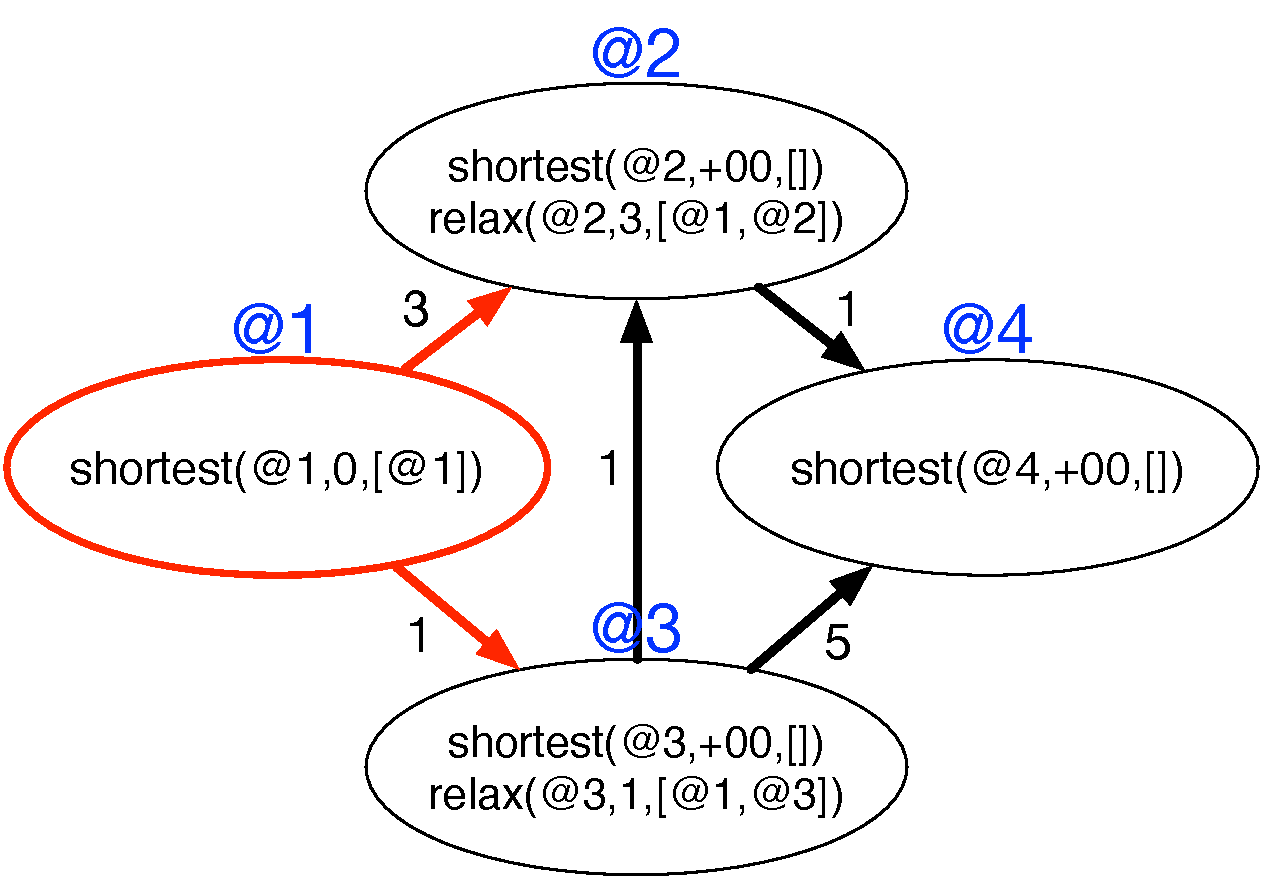
\includegraphics[width=\textwidth]{figures/sssp/shortest2}
   \end{subfigure}
   \begin{subfigure}[b]{0.4\textwidth}
      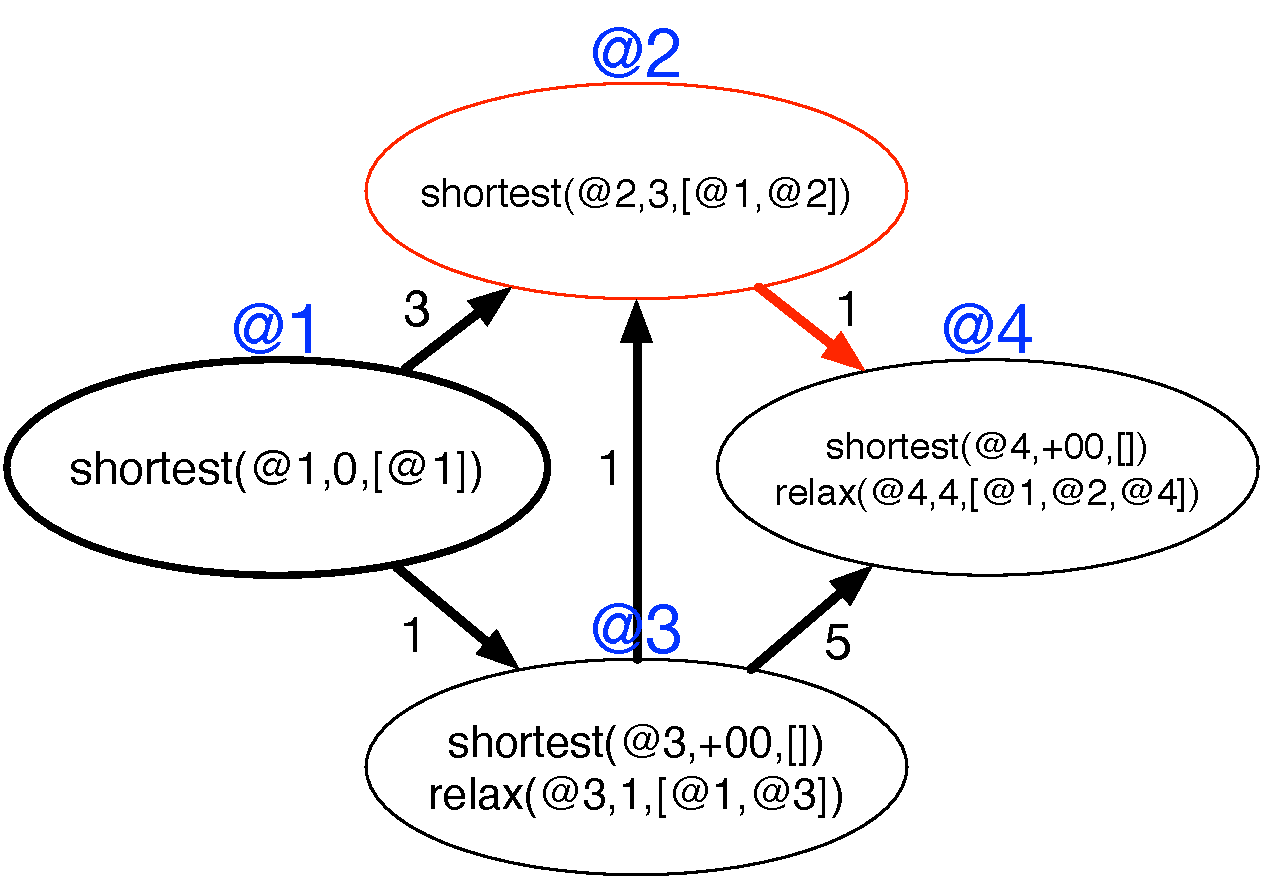
\includegraphics[width=\textwidth]{figures/sssp/shortest3}
   \end{subfigure}
   \begin{subfigure}[b]{0.4\textwidth}
      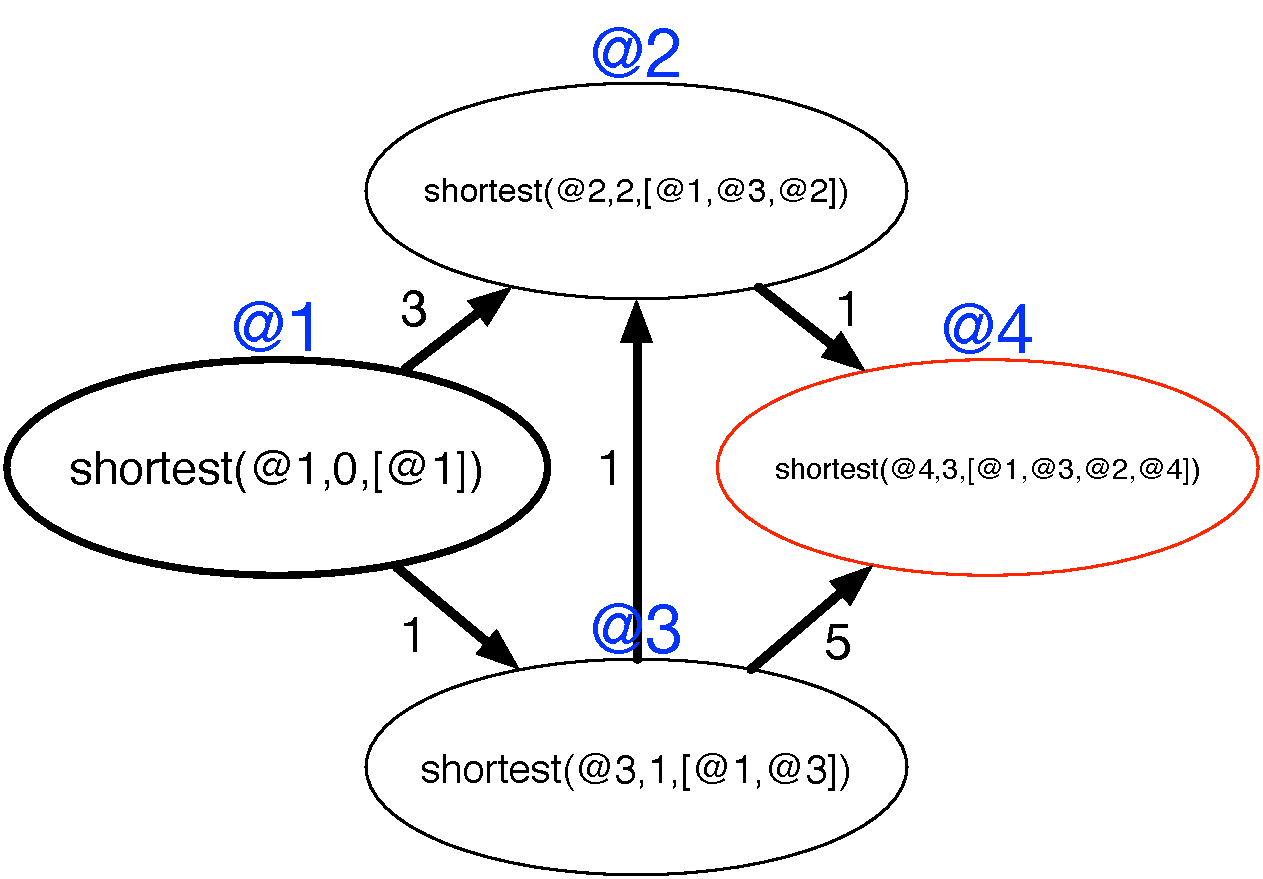
\includegraphics[width=\textwidth]{figures/sssp/shortest8}
   \end{subfigure}
\end{center}
\caption{Graphical representation of the SSSP program. (a) represents the
   program after propagating initial distance at node \texttt{@1}, followed by
   (b) where the first rule is applied in node \texttt{@2}. (c)
   represents the state of the final program, where all the shortest paths
   have been computed.}
\label{fig:shortest_path_program}
\end{figure}

The first rule of the program (lines 11-14) reads as following: if the current
\texttt{shortest} path \texttt{P1} with distance \texttt{D1} is larger than a
new path \texttt{relax} with distance \texttt{D2}, then replace the current
shortest path with \texttt{D2}, delete the new \texttt{relax} path and propagate
new paths to the neighbors (lines 13-14).  The comprehension iterates over the
edges of node \texttt{A} and derives a new \texttt{relax} fact for each node
\texttt{B} with the distance \texttt{D2 + W}, where \texttt{W} is the weight of
the edge. For example, in Fig.~\ref{fig:shortest_path_program}~(a) we apply rule
1 in node \texttt{@1} where two new \texttt{relax} facts are derived at node
\texttt{@2} and \texttt{@3}. Fig.~\ref{fig:shortest_path_program}~(b) is the
result after applying the same rule but at node \texttt{2}.

The second rule of the program (lines 16-17) retracts a \texttt{relax} fact
that has a longer distance than the current shortest distance stored in
\texttt{shortest}.

There are many opportunities for custom scheduling in the SSSP program. For
instance, after applying rule 1 in Fig.~\ref{fig:shortest_path_program}~(a), it
is possible to either apply rules in either node \texttt{@2} or node
\texttt{@3}. This decision depends largely on implementation factors such as
node partitioning and number of threads in the system.  Still, it is easy to
prove that no matter the scheduling used, the final result, as presented in
Fig.~\ref{fig:shortest_path_program}~(c), is achieved.

The SSSP program is concise and declarative but its performance depends on the
order in which nodes are executed. If nodes with greater distances are
prioritized over other nodes, the program will generate more \texttt{relax}
facts since it will take longer to reach the shortest distances. From
Fig.~\ref{fig:shortest_path_program}, it is clear that the best scheduling is
the following: \texttt{@1}, \texttt{@3}, \texttt{@2} and then \texttt{@4}, where
only 4 \texttt{relax} facts are generated. If we had decided to process nodes in
order \texttt{@1}, \texttt{@2}, \texttt{@4}, \texttt{@3}, \texttt{@4},
\texttt{@2}, then 6 \texttt{relax} facts would have been generated.  The optimal
solution for SSSP is to schedule the node with the shortest distance, which is
essentially the Dijkstra shortest path algorithm~\cite{Dijkstra}. Note how it is
possible to change the nature of the algorithm by simply changing the order of
node computation, but still retain the declarative nature of the program.

\section{Types of Facts}

LM introduces the concept of coordination that allows the programmer to write
code that changes how the runtime system schedules and partitions node across
threads of execution. Beyond the distinction between linear and persistent
facts, LM further classifies facts into 3 categories: \emph{computation} facts,
\emph{structural} facts and \emph{coordination} facts.
Predicates are also classified accordingly.

Computation facts are regular facts used to represent the program state. In
Fig.~\ref{code:shortest_path_program}, \texttt{relax} and \texttt{shortest} are
all computation facts.

Structural facts describe information about the connections between the nodes in
the graph.  In the example of Fig.~\ref{code:shortest_path_program},
\texttt{edge} facts are structural since the corresponding \texttt{edge}
predicate is marked as a \texttt{route} predicate. Note that structural facts
can also be seen as computation facts since they are heavily used in the program
logic.

\emph{Coordination facts} allow the programmer to change how the run time
schedules nodes and how it partitions the nodes among threads of execution.
Coordination facts can be used in either the body of the rule, the head of the
rule or both.  This allows scheduling and partition decisions to be made based
on the state of the program and on the state of the underlying machine.  In this
fashion, we keep the language declarative because we reason logically about the
state of execution, without the need to introduce extra-logical operators into
the language that would introduce significant issues when proving properties
about programs.

Coordination facts are further classified into two kinds of facts:
\emph{sensing} and \emph{action} facts. Sensing facts are used to sense
information about the underlying runtime system, including node placement and
node scheduling.  Action facts are used to apply a coordination operations on
the runtime system.

%%%%%%%%%%%%%%%%%%%%%%%%%%%%%%%%%%%%%%%%%%%%%%%%%%%%%%%%%%%%%%%%%%%%%%%%%%%

Sensing facts are facts about the current state of the runtime system, such as
the placement of nodes in the CPU and scheduling information. In the original
Meld, sensing facts were used to get information about the outside world, like
temperature, touch data, neighborhood status, etc.

Action facts are linear facts which are consumed when the corresponding action
is performed.  In the original Meld, they were used to make the robots perform
actions in the outside world.  For LM we use them to change information about
the program state in the user interface. For example, when we want to change the
color of nodes or the label of edges, we just derive a new action fact and the
action is performed in the interface.  A more important use of action facts is
to change the order in which nodes are evaluated in the runtime system. It is
possible to give hints to the virtual machine in order to prioritize the
computation of some nodes.

With sensing facts and action facts, we can write \emph{meta-rules} that will
sense the state of the runtime system and then apply decisions in order to
improve execution speed.  In some situations, this set of rules can be added to
the program without any modifications to the original rules.

\section{Scheduling Facts}

We can use action facts to change the order in which nodes are evaluated by
adding \emph{priorities}. Node priority works at the worker level so that each
worker can make a local decision about which node of the graph to run next.
Note that, by default, nodes are picked arbitrarily (a FIFO approach is used).

The following list presents the action facts available to manipulate the
scheduling decisions of the system:

\begin{description}

   \item[\texttt{type linear action set-priority(node, float)}]: This sets the
      priority of a node. If the node already has some priority, we only change
      the priority if the new one is higher priority. The programmer can decide
      if priorities are to be ordered in ascending or descending order.

   \item[\texttt{type linear action add-priority(node, float)}]: This gets the
      current node's priority and increases or decreases it.

   \item[\texttt{type linear action schedule-next(node)}]: The work will fetch
      the highest priority node's priority $P$ from its set of nodes and set the
      action's argument node's priority as $P + 1.0$. If using the priorities in
      ascending order, we pick the lowest priority and subtract $1.0$.

   \item[\texttt{type linear action unset-priority(node)}]: Removes the
      priority, if any, of a given node.

   \item[\texttt{type linear action stop-program(node)}]: Immediately stops the
      execution of the whole program.

\end{description}

When the highest priority node is picked up for execution, its priority is reset
to 0 (the default priority value). This means that the programmer must set the
node's priority again if he wants to prioritize that node.

We intend to add more action facts in the near future. For example, we want the
programmer to be able to place specific nodes in workers. This will permit good
use of memory locality by forcing certain computations to be performed in the
same worker.

Sensing facts provide information about node placement and node priority. We can
use those facts to express coordination policies. LM provides the following two
sensing facts:

\begin{description}

   \item[\texttt{type linear cpu-id(node, node, int)}]: The third argument
      indicates the worker's ID where the node of the second argument is
      currently running.

   \item[\texttt{type linear priority(node, node, float)}]: The third argument
      is the current priority of the node in the second argument.

\end{description}

Note that when sensing facts are consumed, they are re-derived automatically,
except if the programmer explicitly tells the compiler otherwise. 

\subsection{Global Directives}

We also provide a few global coordination statements:

\begin{description}

   \item[\texttt{priority @order ORDER.}] \texttt{ORDER} can be either
      \texttt{asc} or \texttt{desc}. This defines if node's are to be selected
      by the smallest or the greatest priority, respectively.

   \item[\texttt{priority @initial P.}] The \texttt{initial} statement informs
      the runtime system that all nodes must start with priority $P$.
      Alternatively, the programmer can define an \texttt{set-priority(A, P)}
      axiom.

   \item[\texttt{priority @static.}] The \texttt{static} priority tells the
      runtime system that the partition of nodes among workers is to be used
      until the end of program. 

   %\item[\texttt{priority @cluster TYPE.}] Define what type of graph clustering
   %to use. \texttt{TYPE} can be either \texttt{static}, \texttt{bfs} or
   %\texttt{random}.

\end{description}

\section{Partitioning Facts}

\section{Programs}

To better understand how coordination directives work, we next present some programs that
take advantage of them.

\subsection{Belief Propagation}

\section{Advantages of Coordination}

Randomized and approximation algorithms can obtain significant benefits from
coordination directives because although the final program results will not be
exact, they follow important statistical properties and can be computed faster.
Examples of such programs are PageRank~\cite{Lubachevsky:1986:CAA:4904.4801} and
Loopy Belief Propagation~\cite{Gonzalez+al:aistats09paraml}.

\section{Summary}

In this chapter we presented the current set of coordination directives,
implemented as sensing and action facts. The use of such facilities allows the
programmer to write derivation rules that change how the runtime system
schedules computation thus improving the executing time and possibly the final
program results. As future work, we intend to extend the set of available
directives and write additional programs using coordination.
